\documentclass{paper}

%\usepackage{times}
\usepackage{epsfig}
\usepackage{graphicx}
\usepackage{amsmath}
\usepackage{amssymb}
\usepackage{color}
\usepackage{subcaption}
\usepackage{caption}
\usepackage{morefloats}


% load package with ``framed'' and ``numbered'' option.
%\usepackage[framed,numbered,autolinebreaks,useliterate]{mcode}

% something NOT relevant to the usage of the package.
\setlength{\parindent}{0pt}
\setlength{\parskip}{18pt}


\usepackage[latin1]{inputenc} 
\usepackage[T1]{fontenc} 

\usepackage{listings} 
\lstset{% 
   language=Matlab, 
   basicstyle=\small\ttfamily, 
} 


\title{Report Computer Vision Project 3}

\author{Single Michael\\08-917-445}
% //////////////////////////////////////////////////


\begin{document}


\maketitle


\section{Video search with bags of visual words}
For generating the data sets for this project I used two $\emph{mp4}$ movies. The first is a sequence of a $\emph{Breaking Bad}$ episode (called $\emph{breakingbad2}$) and the second is a demo video found used for various purposes showing some kids playing with their toys 
(called $\emph{test\_video}$). These video files are stored in the folder \emph{video/}. \\

I extracted from each movie their frames and stored them as png images in \emph{frames/} using my Matlab function \emph{extractVideoFrames}. For each frame converted to a grayscale image, I computed its corresponding SIFT data using VLFeat's function \emph{vl\_sift}.
Hence, for each extracted frame I create a \emph{.mat} file that contains 

\begin{itemize}
    \item the SIFT vectors (encoded in the rows)
    \item the name of the frame.
    \item the number of detected features
    \item the orientation of the patches
    \item the positions of the patch center.
    \item the scales of the patches.
\end{itemize}

You can generate your own mat files using my function \emph{computeSiftDataOf}. \\

Last, I additionally assembled all mat files into one big mat file, which contains all mat files in a sequential order. This is just to simplify the coding that had to be done for the assignment. You can find all those mat files in the folder \emph{data/}. \\

\subsection{Raw Descriptor Matching}
Note: run the script \emph{rawDescriptorMatches} in order to reproduce my results. \\

First we load the precomputed SIFT data of two chosen images (called left and right) from our data sets. Then we let a user select a region (relying on the provided script \emph{selectRegion}) in the left image. Each point within the user-selection is then considered as a feature point in the left image. \\

Next we try to match these left-image feature points to corresponding, closest feature points in the right image. For the matching process, we calculate the distance (2-norm) between the descriptors of the left features with all possible descriptors from the left image (Remember: those descriptors are stored in the corresponding mat files). In practise we compute the distance between all possible descriptor pair combinations where the first points is from the left descriptor and the second point is from the right descriptor (using the provided \emph{dist2} function) and store those distances in a $M \times N$ matrix D. Note that the m-th row in $D$ corresponds to the m-th element in the left descriptor and the n-th colum in $D$ corresponds to the n-th element in the right descriptor. \\

For each row, we look for the minimum element, i.e. the minimum distance. This corresponds to finding the column which has the smallest distance value for a fixed row. Since a column index corresponds to the same index in the right descriptor, this retrieved column index corresponds to the best matching feature point index in the right descriptor matching to a given descriptor point in the left image (i.e. for a given row index). \\

Since we only are interested in good matching feature point pairs, we introduce an additional constraint. Each determined minimum is taken if and only if it is still the minimum distance in its row, when being scaled by a certain factor that depicts a acceptance parameter. This factor has to be bigger than one. This ensures, that we only take strong and reliable matchings. This also implies that not every descriptor point in the right image has a corresponding point in the left image. \\

In practise we first look for the minimum distance index in each row. We store these minima and their indices as candidates in an array and then set their values in $D$ equal to infinite. We than again look for the minimum value in this updated $D$ matrix. This will give us the second smallest distance value column-index for each row. We then compare the initial candidate minima scaled by a user specified acceptance value with the second smallest retrieved minima values. If the scaled candidates are still smaller than the second smallest minima (unscaled), then we have found a true minimum otherwise we discard this candidate. \\

In my code I set this scale equal to two, i.e. if twice the minimum is still smaller than the second smallest row distance, then we have found a true minimum (index), i.e. we have found a matching. So every index pair (row column) of such a true minimum is a matching pair, where the first element corresponds to the left and the second element to the right feature point. \\

For each feature points we look up its SIFT data, i.e. their position, scale and orientation. We pass those values to the provided function \emph{displaySIFTPatches} and hereby show the corresponding matches in the left and right images (resulting by the given user-selection). \\

In the following I show my results I got using my implementation. My first example shows the results of the \emph{twoFrameData} data-set that acts as a test case for my implementation. Similarly as shown in the exercise sheet I selected the upper door of the fridge and got similar results shown in FIGURE. Figure $\ref{fig:friends_raw_sel}$ shows the feature points in the left image and figure $\ref{fig:friends_raw_matching}$ shows the corresponding matching points in the right image. \\

I applied this feature matching the same way to my own data-sets. 

\begin{itemize}
    \item Breaking Bad data set: White tubus selection shown in figure $\ref{fig:friends_raw_sel}$ and the matching shown in figure $\ref{fig:bb_raw_matching}$.
    \item Kids data set: Selection of boy's t-shirt shown in figure $\ref{fig:kids_raw_sel}$ and their matchings shown in figure $\ref{fig:kids_raw_matching}$.
    \item Kids data set: Selection of collection of toys shown in figure $\ref{fig:kids2_raw_sel}$ and the corresponding matchings shown in figure $\ref{fig:kids_raw_matching}$.
\end{itemize}

In summary, the matching produced in my implementation seems to work.

% friends data-set
\begin{figure}[H]
\centering
\begin{subfigure}{1.0\textwidth}
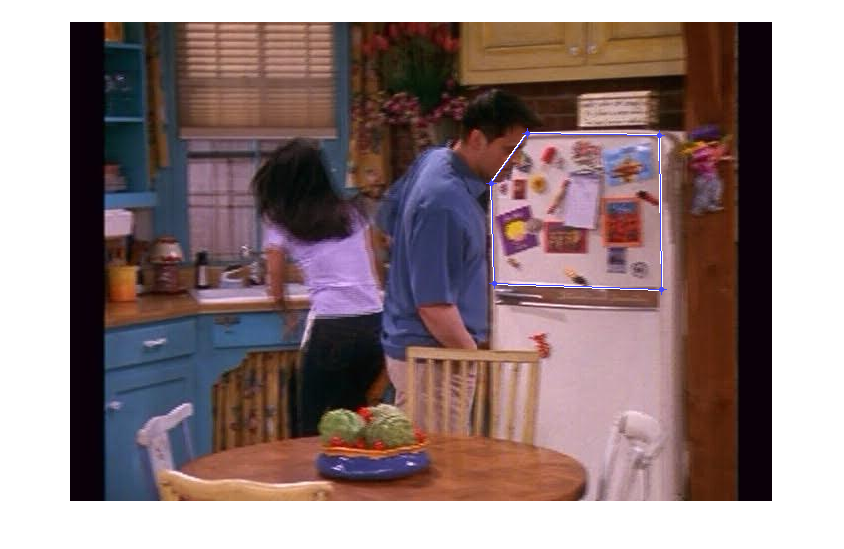
\includegraphics[width=\textwidth]{figures/raw_matches/friends/friendsSelection}
\end{subfigure}
\caption{User selection in left image of provided twoFramesData data set.}
\label{fig:friends_raw_sel}
\end{figure}

\begin{figure}[H]
\centering
\begin{subfigure}{1.0\textwidth}
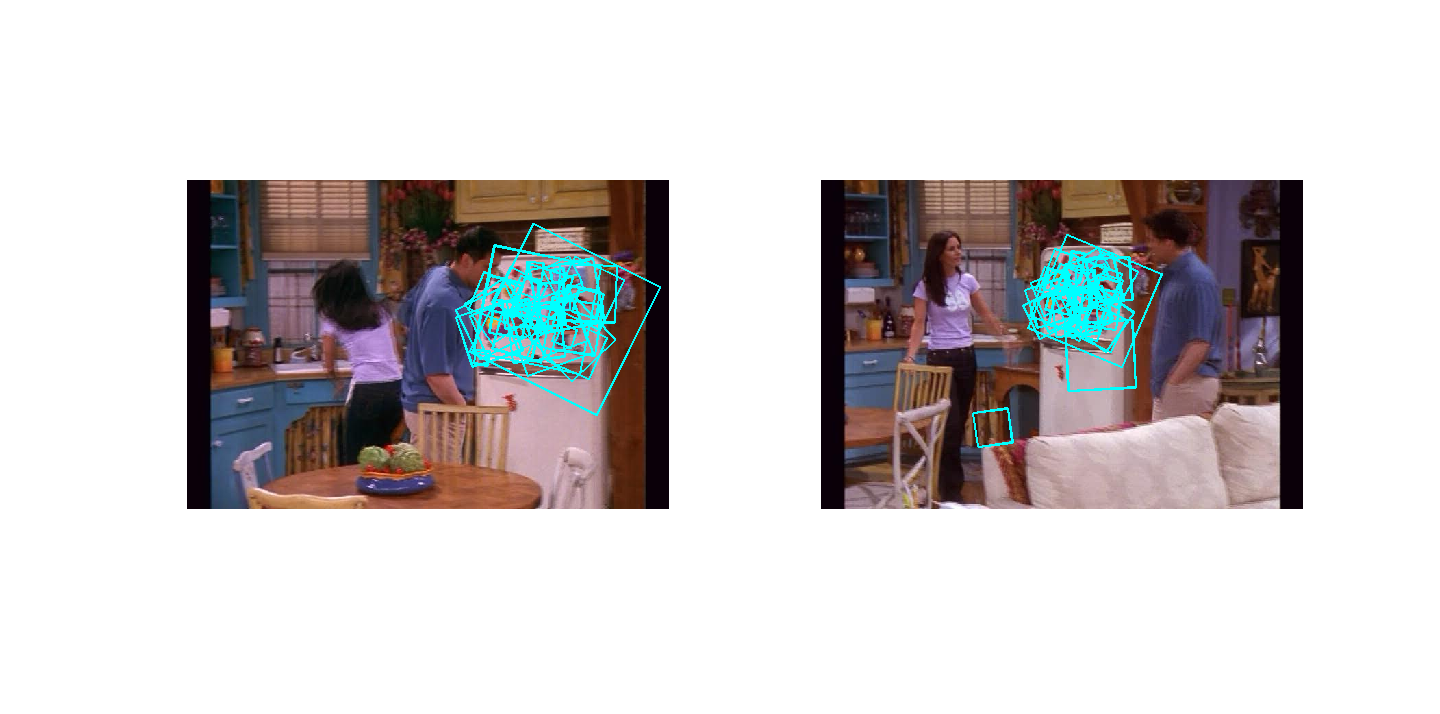
\includegraphics[width=\textwidth]{figures/raw_matches/friends/friendsMatches}
\end{subfigure}
\caption{On the left feature points in the user specified selection region and on the right the their matched feature points.}
\label{fig:friends_raw_matching}
\end{figure}

% breaking bad data-set
\begin{figure}[H]
\centering
\begin{subfigure}{1.0\textwidth}
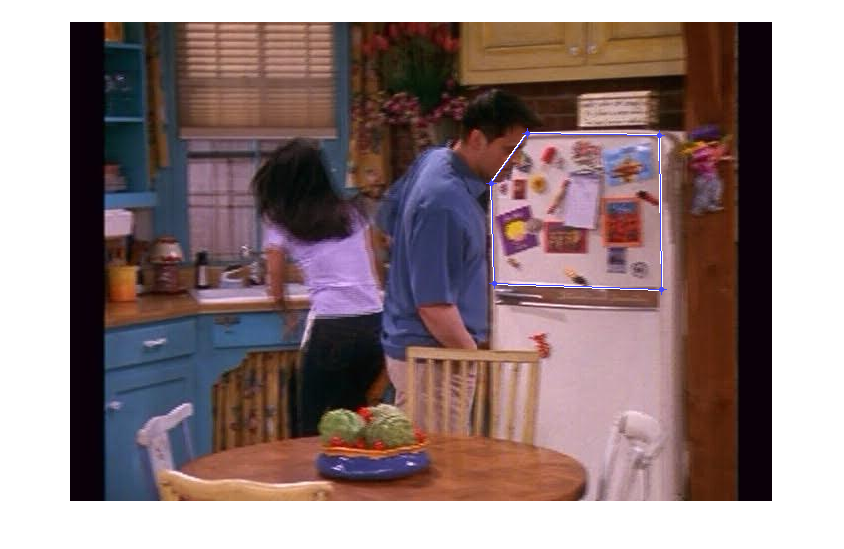
\includegraphics[width=\textwidth]{figures/raw_matches/friends/friendsSelection}
\end{subfigure}
\caption{User selection in left image of provided twoFramesData data set.}
\label{fig:friends_raw_sel}
\end{figure}

\begin{figure}[H]
\centering
\begin{subfigure}{1.0\textwidth}
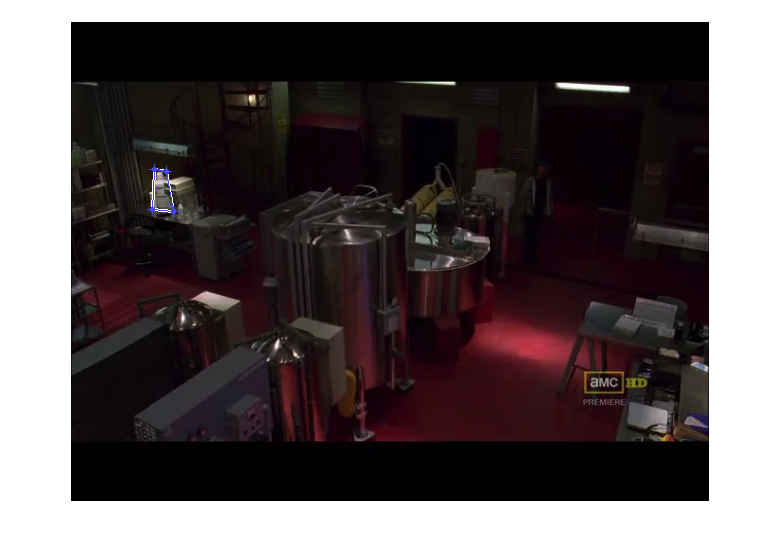
\includegraphics[width=\textwidth]{figures/raw_matches/bb/breakingBadRawSelection_1}
\end{subfigure}
\caption{On the left feature points in the user specified selection region and on the right the their matched feature points.}
\label{fig:bb_raw_matching}
\end{figure}

% kids data-set
\begin{figure}[H]
\centering
\begin{subfigure}{1.0\textwidth}
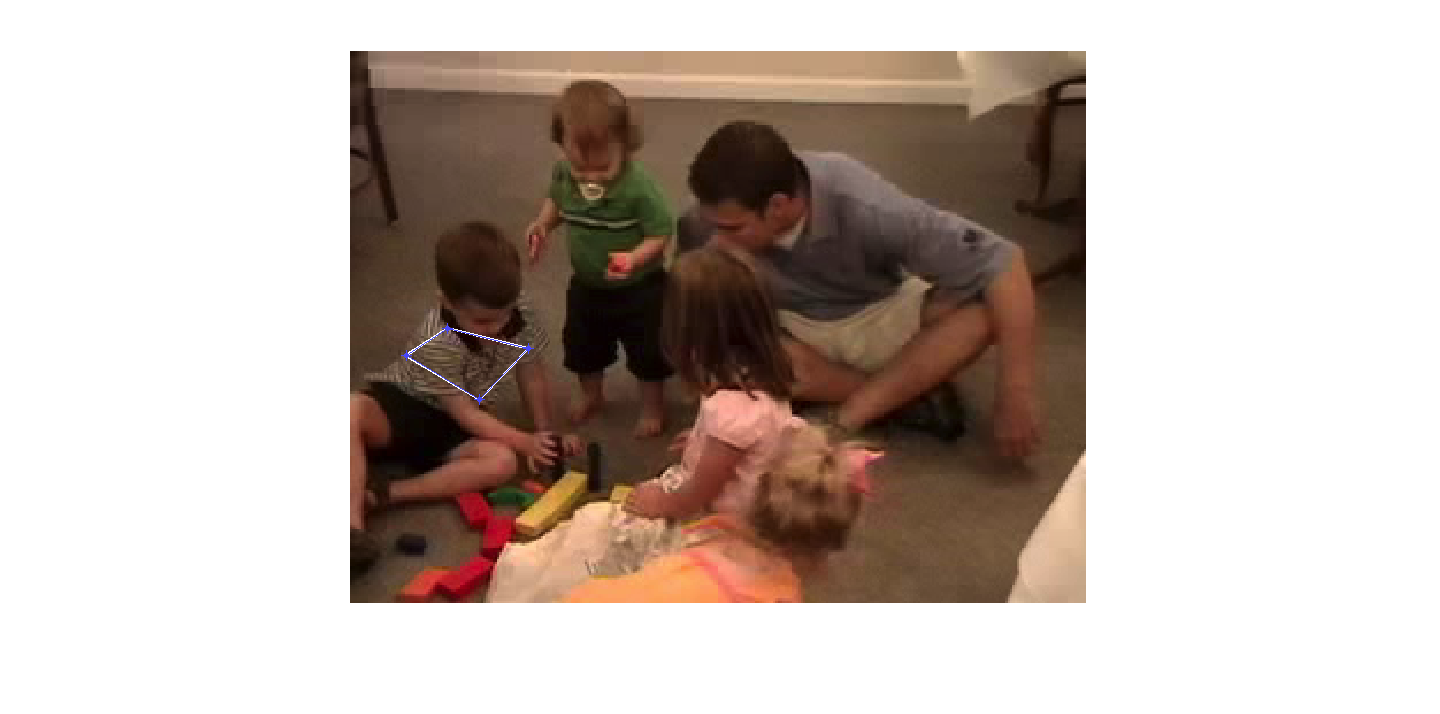
\includegraphics[width=\textwidth]{figures/raw_matches/kids/selMatch1}
\end{subfigure}
\caption{User selection in left image of provided twoFramesData data set.}
\label{fig:kids_raw_sel}
\end{figure}

\begin{figure}[H]
\centering
\begin{subfigure}{1.0\textwidth}
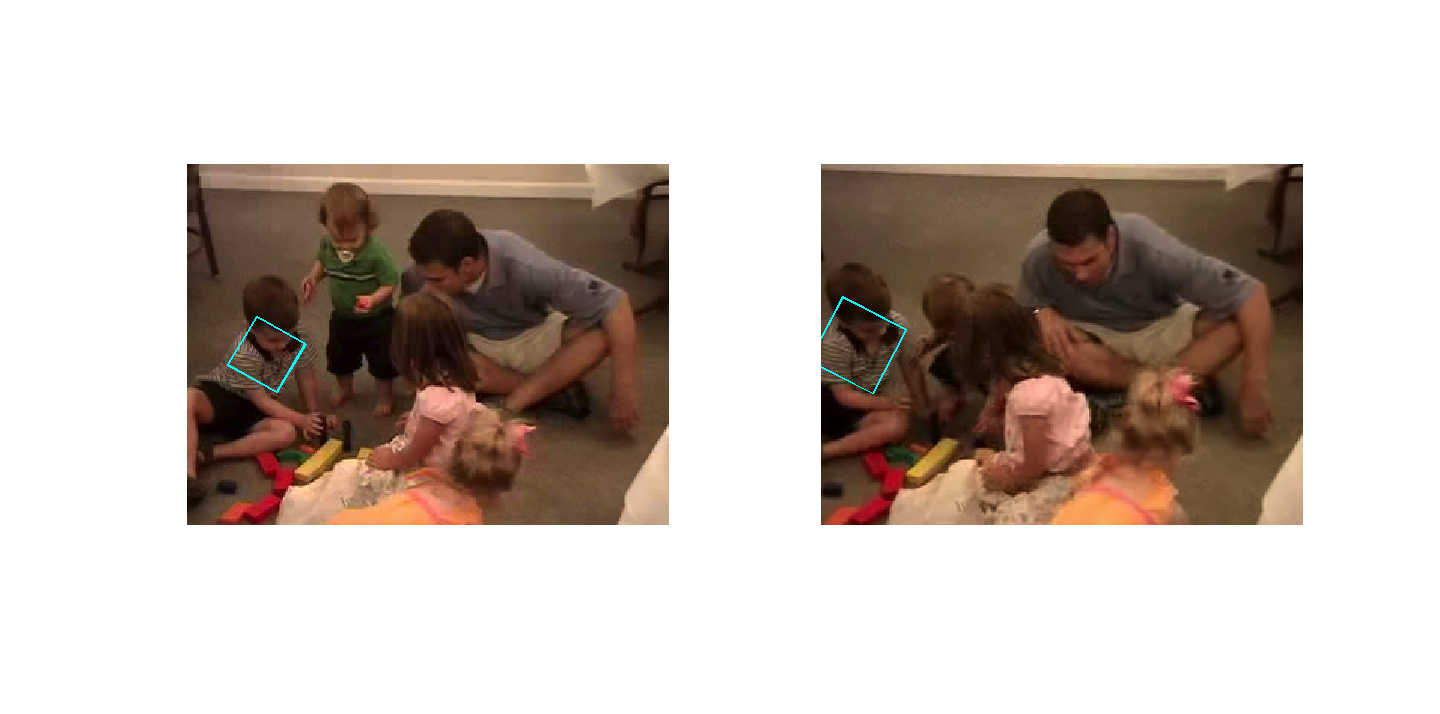
\includegraphics[width=\textwidth]{figures/raw_matches/kids/match1}
\end{subfigure}
\caption{On the left feature points in the user specified selection region and on the right the their matched feature points.}
\label{fig:kids_raw_matching}
\end{figure}

% kids2 data-set
\begin{figure}[H]
\centering
\begin{subfigure}{1.0\textwidth}
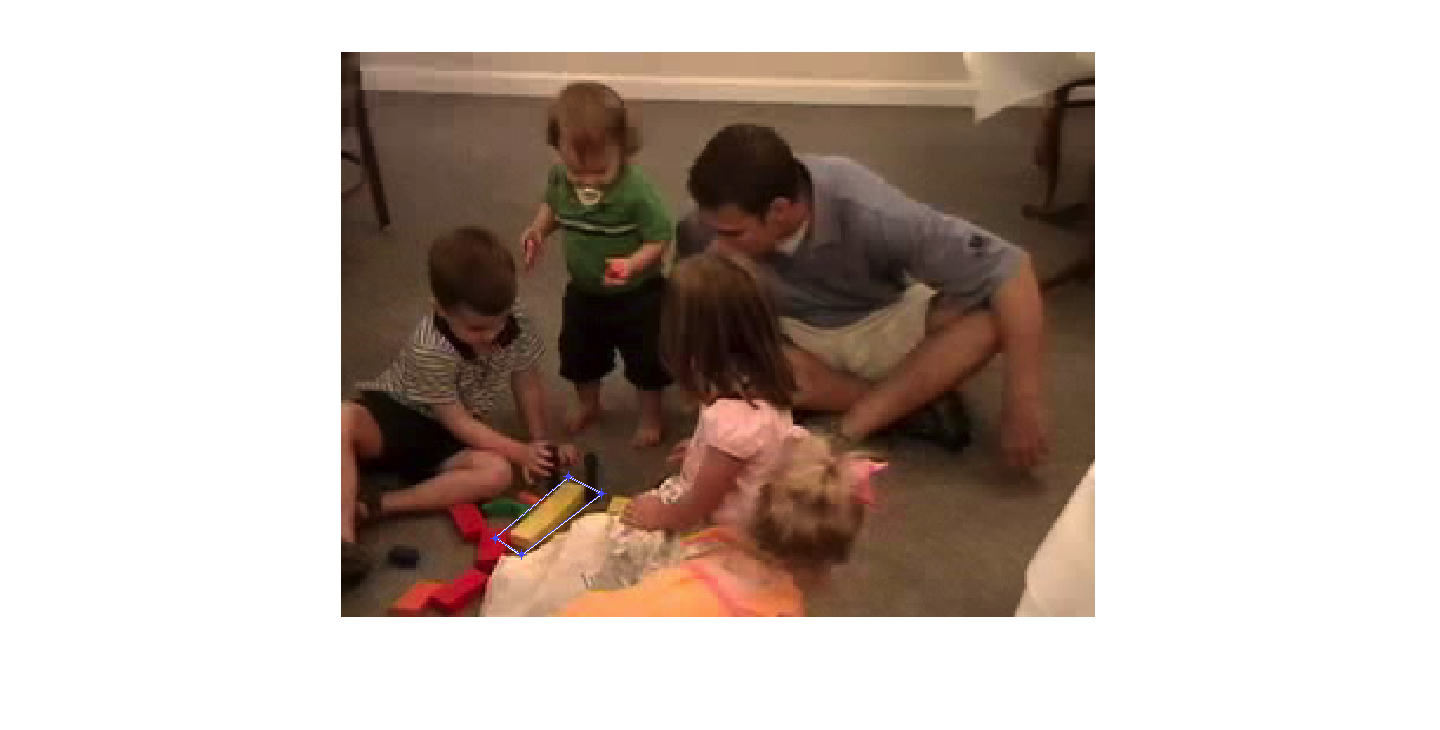
\includegraphics[width=\textwidth]{figures/raw_matches/kids/selMatch2}
\end{subfigure}
\caption{User selection in left image of provided twoFramesData data set.}
\label{fig:kids2_raw_sel}
\end{figure}

\begin{figure}[H]
\centering
\begin{subfigure}{1.0\textwidth}
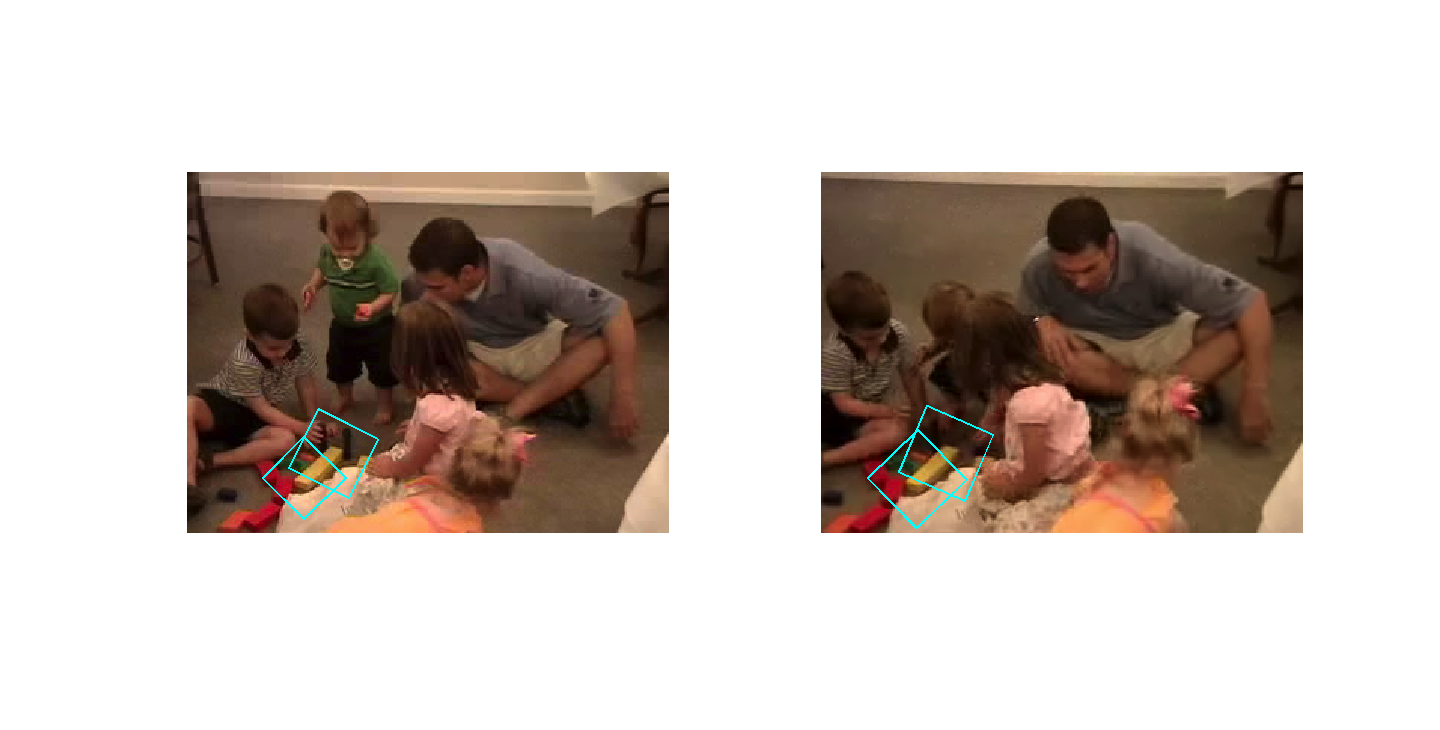
\includegraphics[width=\textwidth]{figures/raw_matches/kids/match2}
\end{subfigure}
\caption{On the left feature points in the user specified selection region and on the right the their matched feature points.}
\label{fig:kids_raw_matching}
\end{figure}



\subsection{Visualizing The Vocabulary}
Note: run the script \emph{visualizeVocabulary} in order to reproduce my results. \\

The goal of this task was to visualize patches associated with two of the visual words, i.e. we are interested in showing the visual vocabulary. This can be achieved by clustering all feature points of all descriptors of a given data-set. For this purpose I use the assembled mat file that has been generated after the generation of the SIFT data of each extracted video frame. This file contains all SIFT data of every frame in a sequential order that belongs to the same data-set. \\

After loading all the SIFT data of every frame, especially all the descriptors (containing all the feature points), I pass that huge set of descriptors to the provided method \emph{kmeansML}. Basically, this method separates all the descriptors (feature points) into k (this is a user specified constant, for this assignment k is equal to 1500) clusters. Each cluster represents a so called word. In the clustering process, each feature points was classified to a particular word. Thus, when selecting a random word, we can retrieve the corresponding feature points that belong to that cluster. From this feature point set, we select 25 of them. From those feature points, we select their corresponding patches from the image using the provided Matlab function \emph{getPatchFromSIFTParameters} and visualize all these patches. \\

In the following I show for each of my data-sets two word visualizations:
\begin{itemize}
    \item Breaking Bad data-set: First visual word example shown in figure $\ref{fig:bb_word_1}$ and second example shown in figure $\ref{fig:bb_word_2}$. The first word clusters features that are associated to a patch showing some kind of cabinet with a tubus and the second word aggregates patches that also look very similar (tubus shaped geometry on the right top corner or a bar-like shape on the top right center).
    \item kids data-set: First visual word example shown in figure $\ref{fig:kids_word_1}$ and second example shown in figure $\ref{fig:kids_word_2}$. The first word aggregates patches that belong to features that look like a arm and the is the word that aggregates features that have a patch showing the head of the man playing with the kids (rotated by 180 degree).
\end{itemize}

We observe that all feature point patches that belong to the same word look similar to each other. The exhibit the same kind of visual appearance in their detail. This holds true for both data sets.


% breaking bad data set
\begin{figure}[H]
\centering
\begin{subfigure}{1.0\textwidth}
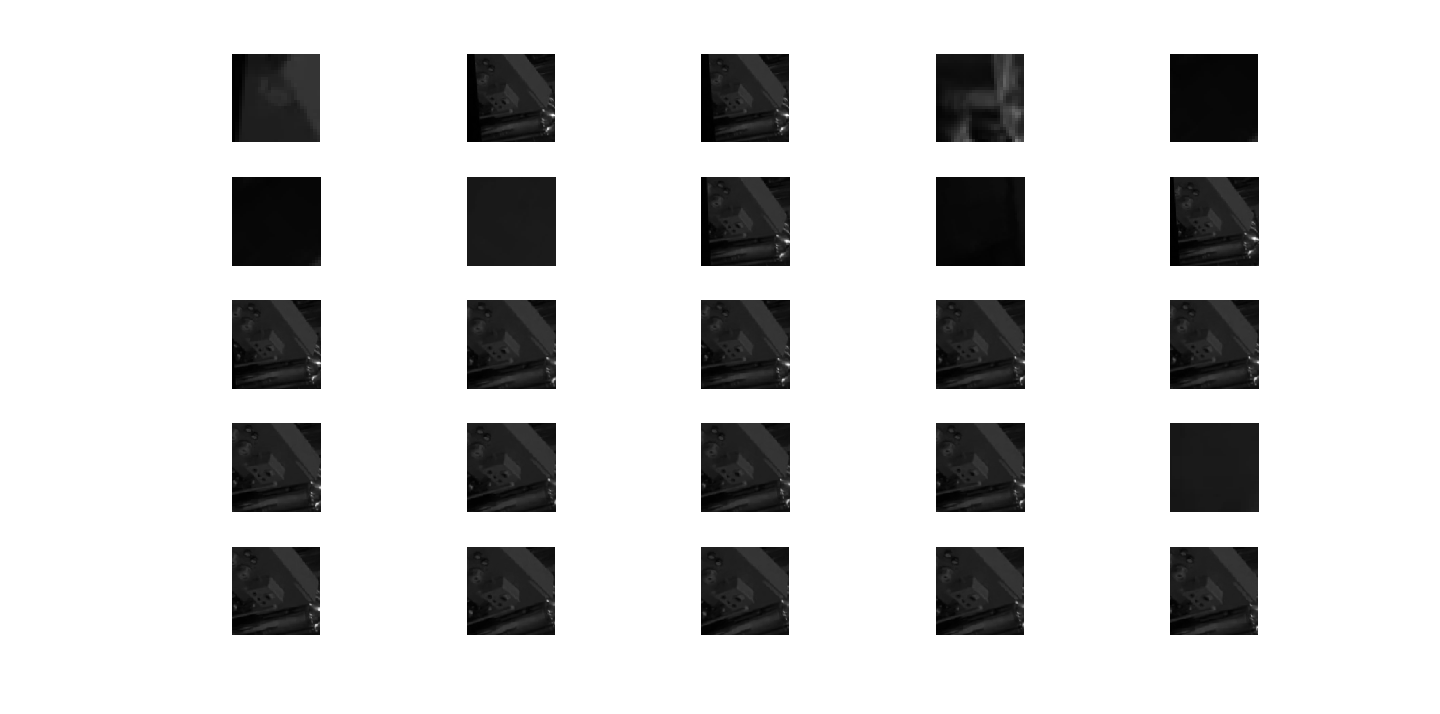
\includegraphics[width=\textwidth]{figures/vocabulary/bb/bbVoca122}
\end{subfigure}
\caption{Breaking Bad data-set: Patches of feature points that belong to the same cluster.}
\label{fig:bb_word_1}
\end{figure}

\begin{figure}[H]
\centering
\begin{subfigure}{1.0\textwidth}
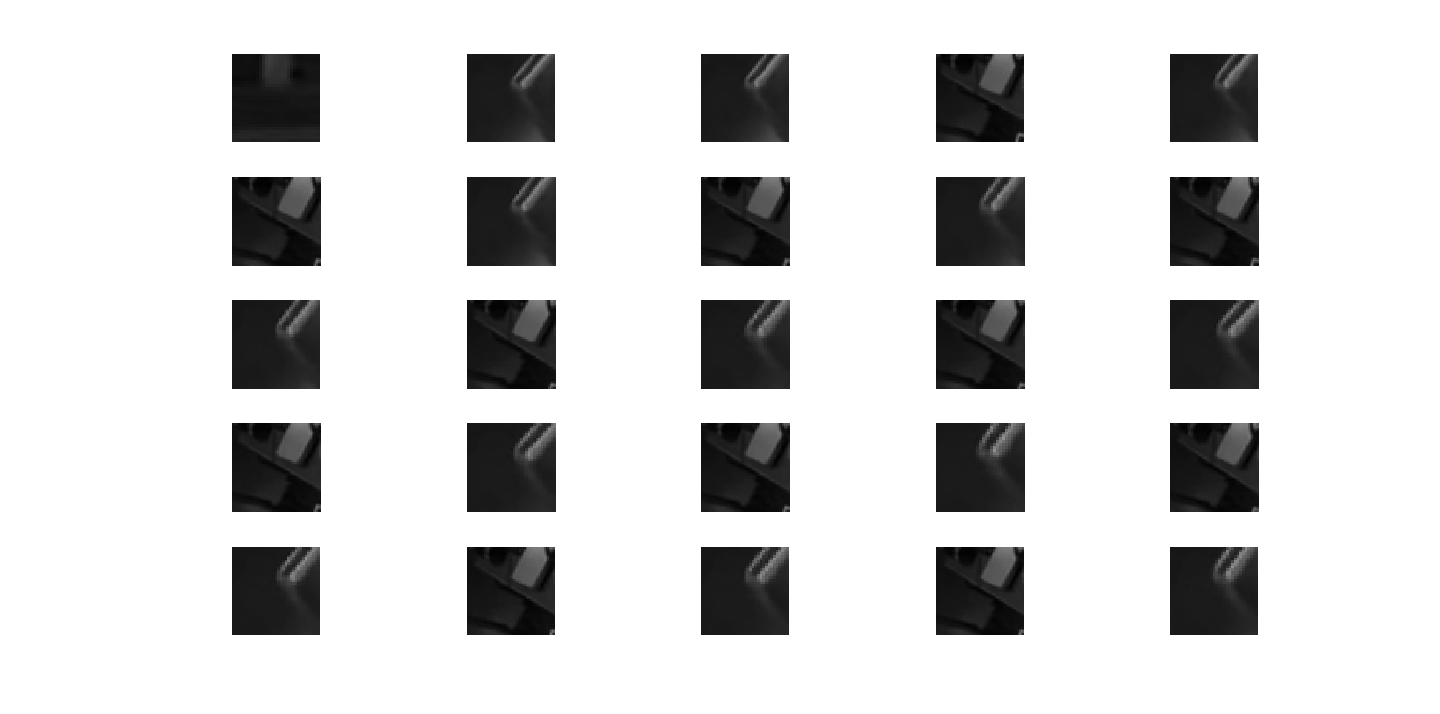
\includegraphics[width=\textwidth]{figures/vocabulary/bb/bbVoca1174}
\end{subfigure}
\caption{Breaking Bad data-set: Patches of feature points that belong to the same cluster.}
\label{fig:bb_word_2}
\end{figure}

% kids data set
\begin{figure}[H]
\centering
\begin{subfigure}{1.0\textwidth}
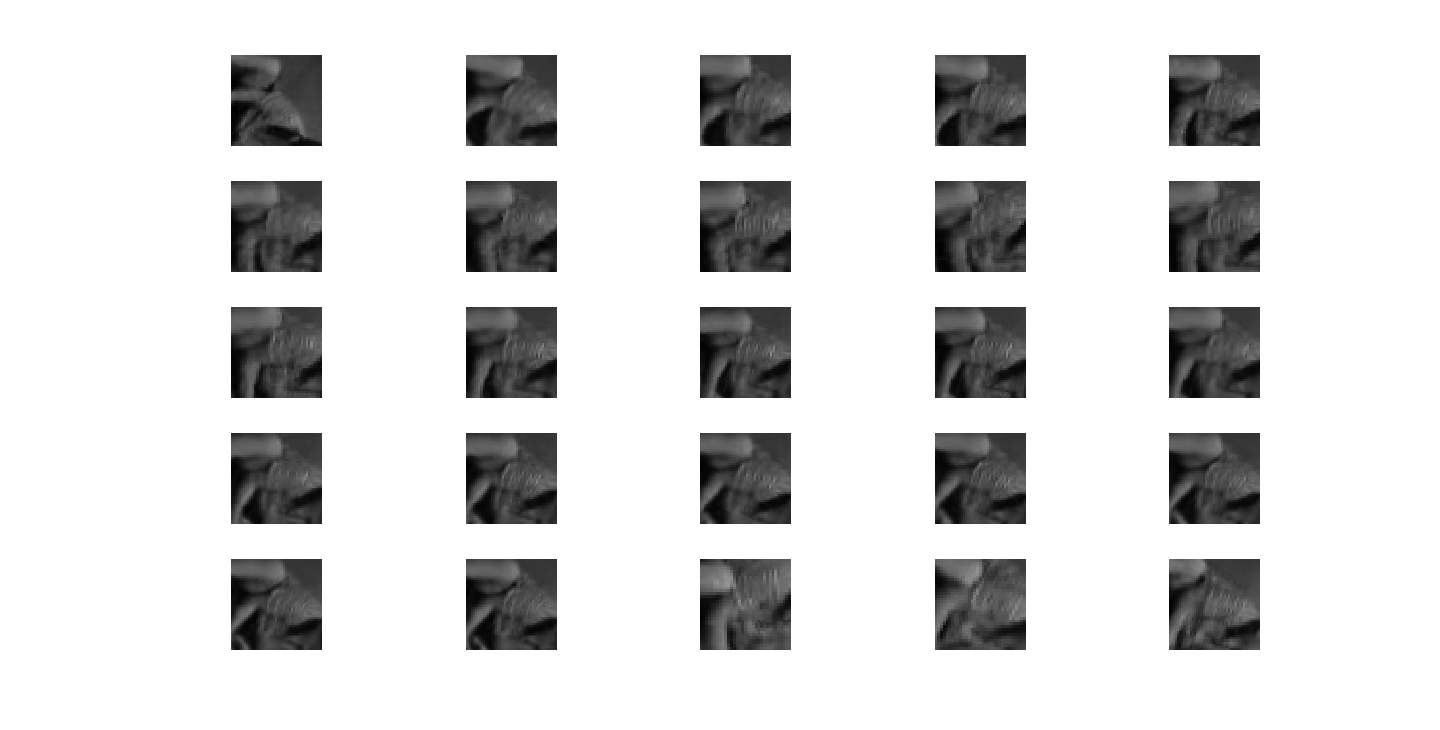
\includegraphics[width=\textwidth]{figures/vocabulary/kids/voca888}
\end{subfigure}
\caption{Kids data-set: Patches of feature points that belong to the same cluster.}
\label{fig:kids_word_1}
\end{figure}

\begin{figure}[H]
\centering
\begin{subfigure}{1.0\textwidth}
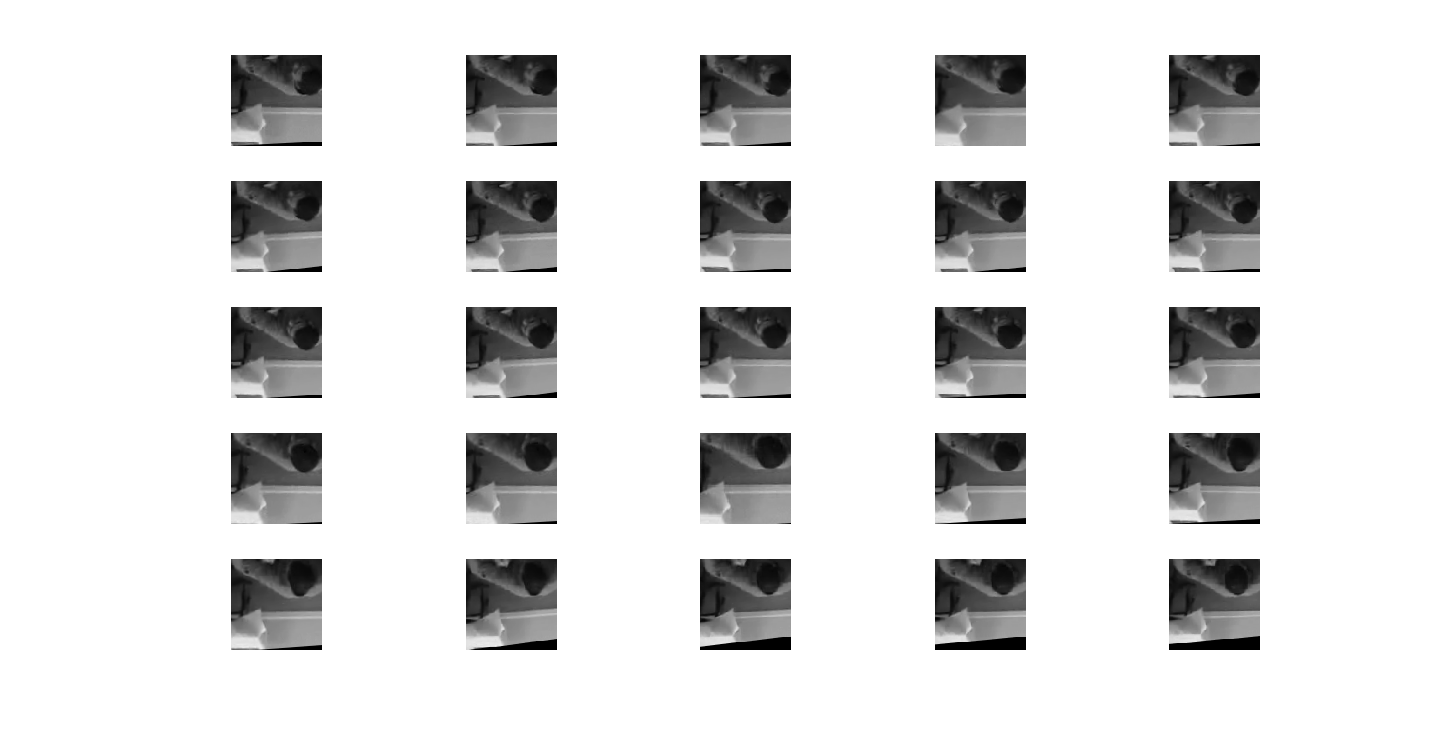
\includegraphics[width=\textwidth]{figures/vocabulary/kids/voca1302}
\end{subfigure}
\caption{Kids data-set: Patches of feature points that belong to the same cluster.}
\label{fig:kids_word_2}
\end{figure}

\subsection{Full Frame Queries}
Note: run the script \emph{fullFrameQueries} in order to reproduce my results. \\

In order to solve this task we again first compute bag of words by clustering all feature points in the set of all descriptors of a data-set of choice. Similarly, as in the previous task we initially load all assembled SIFT data of the frames belonging to target data-set. We then perform the clustering of the descriptor features as we did before. \\

Next, we compute a histogram of all frames, indicating how many words belong to a particular cluster. I.e. we count how many features are classified to a certain cluster. For this purpose, we technically rely on the descriptors of frame and apply Matlab's \emph{histc} function. \\

Next we choose a random frame and compare its histogram to the histograms of all other frames. For comparing the selected histogram by any other histogram (i.e. applying a measure), we compute the normalized scalar product between them. This gives us a number between zero and one. The closer the result, the more identical the two histograms are. This implies that two histograms are the same, if their normalized scalar product is equal to one and they are completely different in case their product is equal zero. We denote their similarity value by the variable \emph{score}. \\

Last, we want to display the 5 most similar frames. By sorting all the similarity scores in a descending order, we simply have to pick those frames that belong to the first five scores in the sorted score set. \\

In my results, the first image is the random selected frame, and all other frames represent depict the frames with the highest scores matching this random frame.

In the following I demonstrate the results when applying the \emph{fullRegionQuery} script to my two data-sets:  

\begin{itemize}
    \item breaking bad data-set: Example one is shown in figure $\ref{fig:bb_fullquery_1}$ and example two is shown in figure $\ref{fig:bb_fullquery_2}$.
    \item kids data-set: Example one is shown in figure $\ref{fig:kids_fullquery_1}$ and example two is shown in figure $\ref{fig:kids_fullquery_2}$.
\end{itemize}

Observation: Frames that are close in time to the selected frame achieve a high score value. In other words, frames that are close in a temporal sequence to the reference frame (i.e. their temporal distance is small) achieve usually a higher score value than frames in later times. This makes sense, since one movie second consists of many frames (approx. 24 frames per second). Within one second, usually, for ordinary sceneries there is not a huge spatial variation between a frame and its successor frame. Therefore, a successor frame is usually very similar to its predecessor frame and thus achieves a large similarity value. However, there are some exceptions, if there suddenly occurs some kind of occlusion for example. then a successor frame will not be close to its parent frame.

% breaking bad data set
\begin{figure}[H]
\centering
\begin{subfigure}{1.0\textwidth}
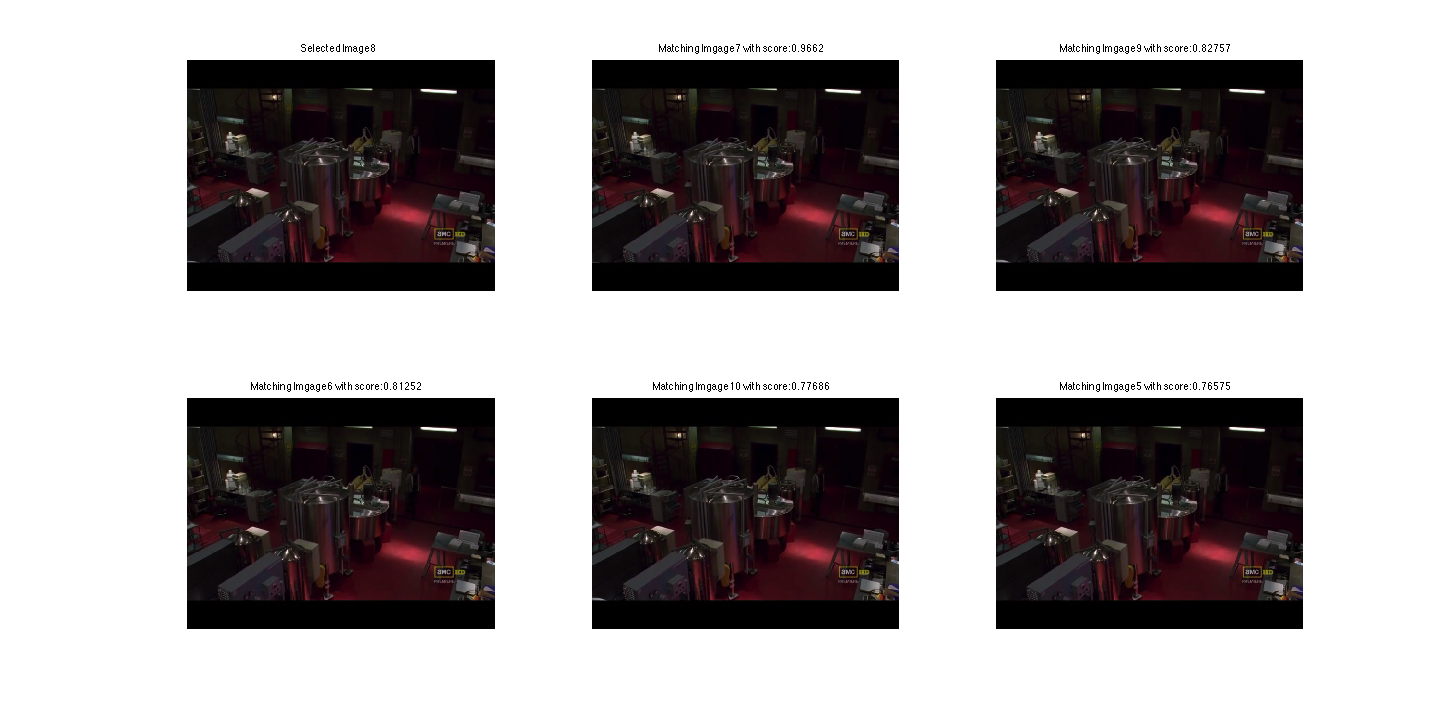
\includegraphics[width=\textwidth]{figures/full_frame_queries/bb/fullQueries8}
\end{subfigure}
\caption{Full Frame Query matchings when selecting frame 8 when using the breaking bad data-set.}
\label{fig:bb_fullquery_1}
\end{figure}

\begin{figure}[H]
\centering
\begin{subfigure}{1.0\textwidth}
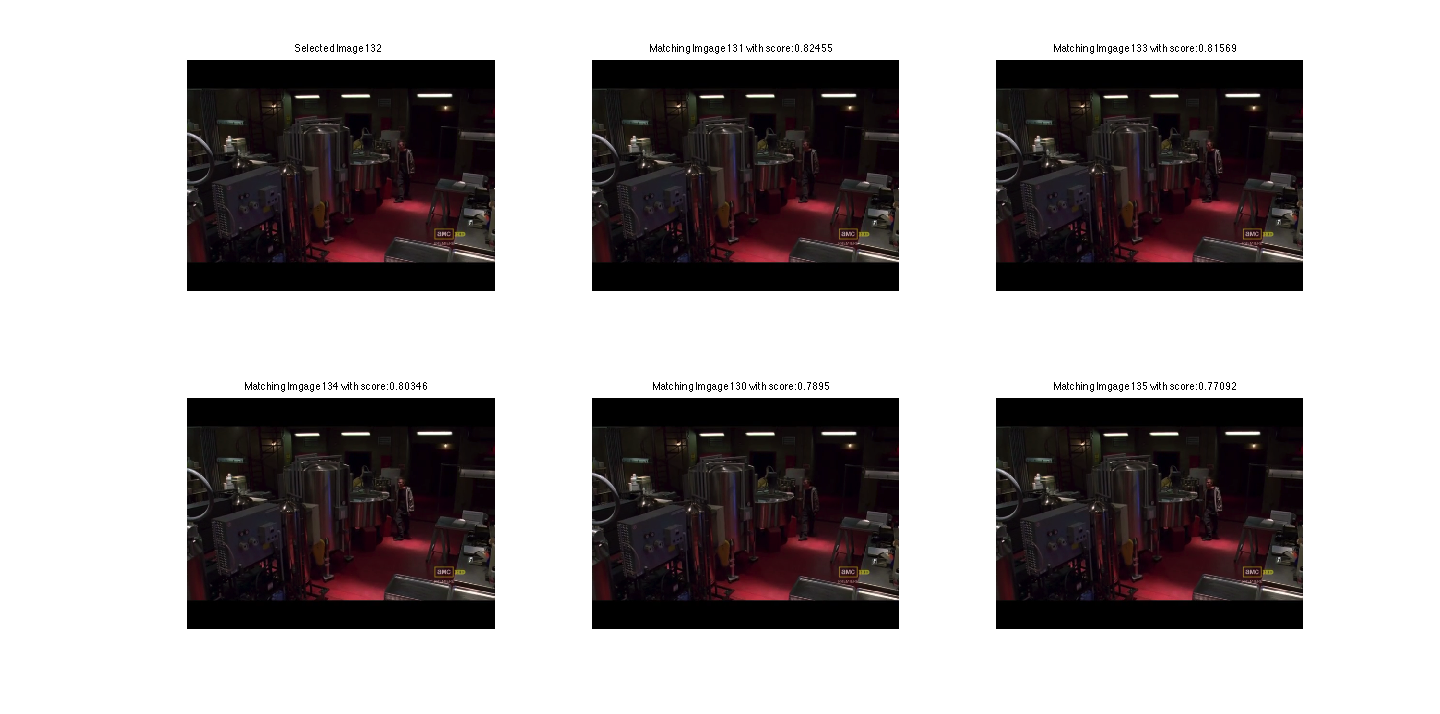
\includegraphics[width=\textwidth]{figures/full_frame_queries/bb/fullQueries132}
\end{subfigure}
\caption{Full Frame Query matchings when selecting frame 132 when using the breaking bad data-set.}
\label{fig:bb_fullquery_2}
\end{figure}

% kids data set
\begin{figure}[H]
\centering
\begin{subfigure}{1.0\textwidth}
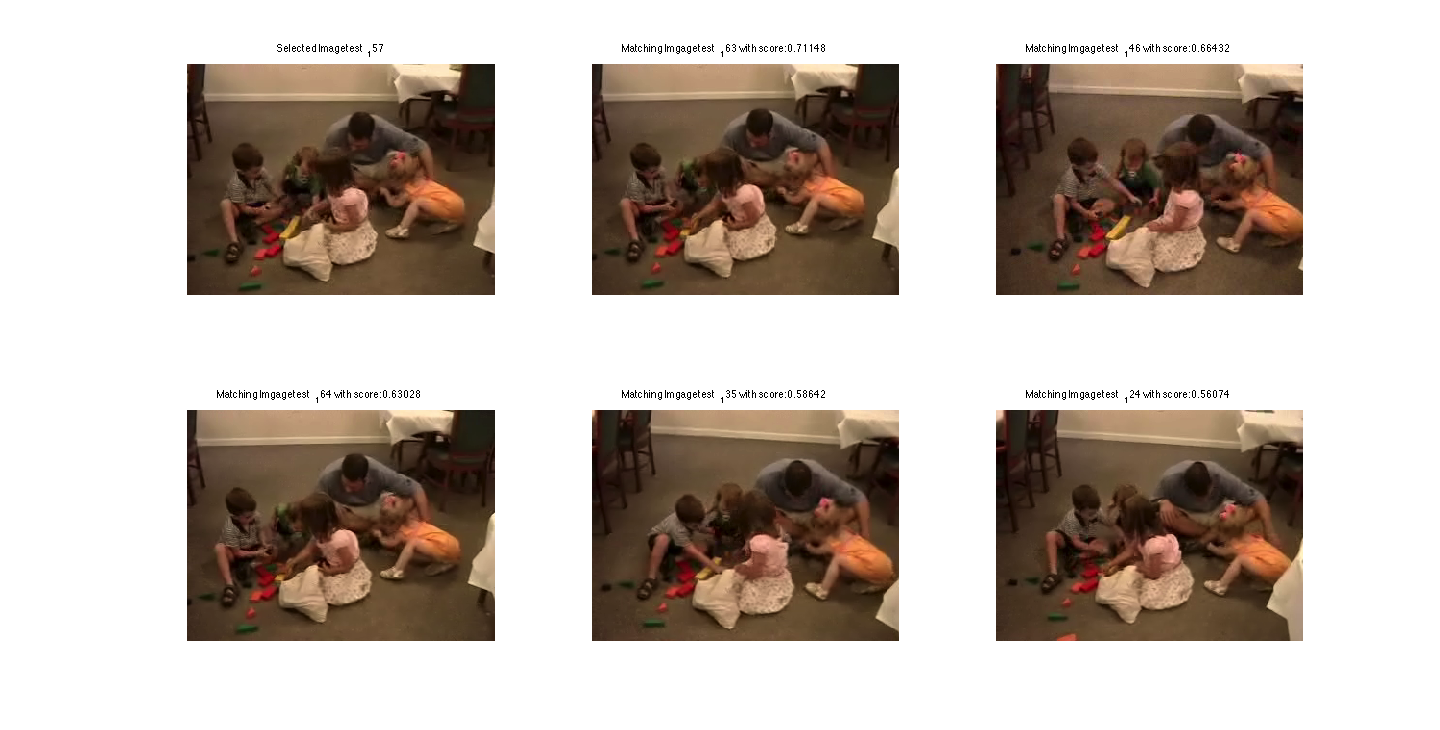
\includegraphics[width=\textwidth]{figures/full_frame_queries/kids/fullQueries157}
\end{subfigure}
\caption{Full Frame Query matchings when selecting frame 157 when using the kids data-set.}
\label{fig:kids_fullquery_1}
\end{figure}

\begin{figure}[H]
\centering
\begin{subfigure}{1.0\textwidth}
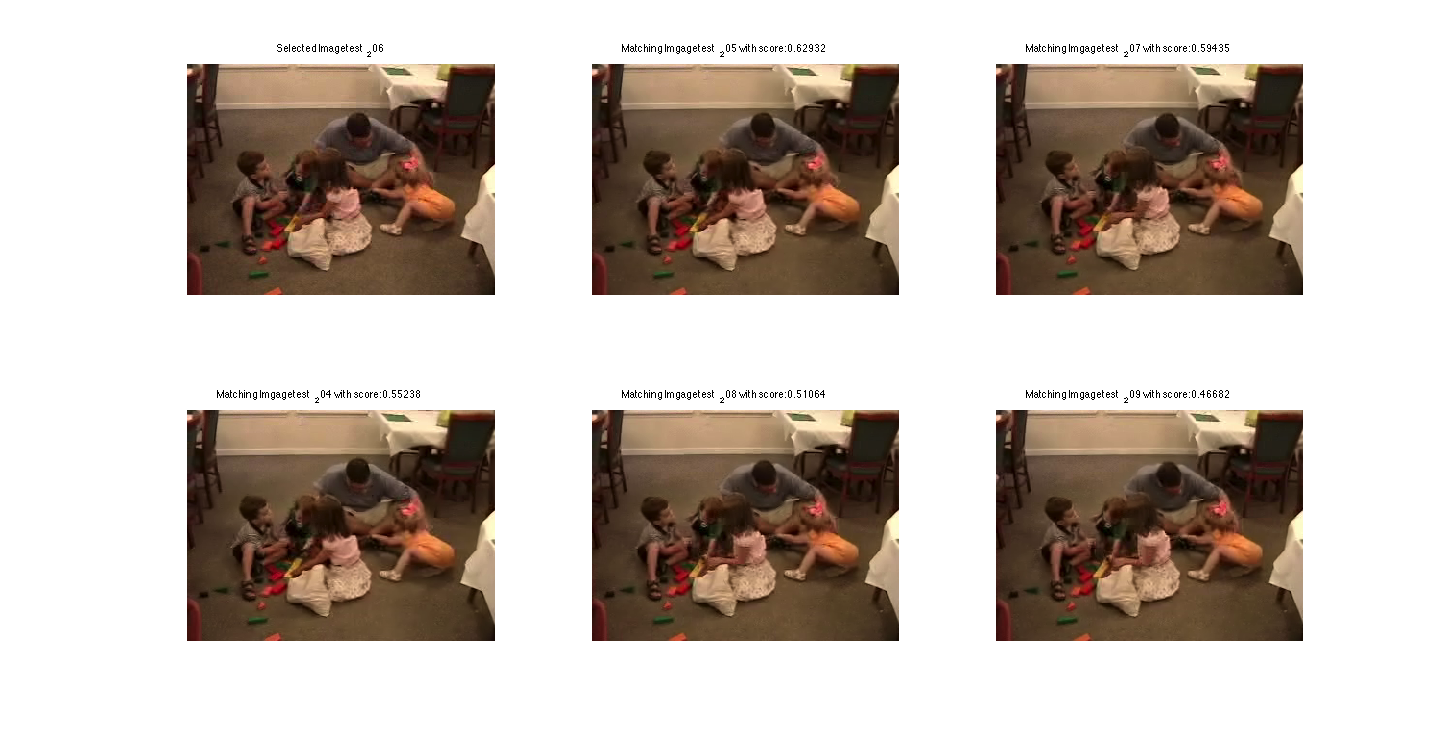
\includegraphics[width=\textwidth]{figures/full_frame_queries/kids/fullQueries206}
\end{subfigure}
\caption{Full Frame Query matchings when selecting frame 206 when using the kids data-set.}
\label{fig:kids_fullquery_2}
\end{figure}

\subsection{Region Queries}
Note: run the script \emph{regionQueries} in order to reproduce my results. \\

First, we compute the bag of words, i.e. vocabulary resulting from the descriptor clustering. We use the same parameters as we did for solving task 3. Then, the user can specify a region of interest in a randomly chosen frame. This corresponds to somehow to task 1. All points within this user selected area are supposed to denote feature points of interest. We select all feature in the frame's descriptor within the selected region and compute their histogram, similarly as we did for task 3. Then we process like we did for solving task 3. We compute the histogram of all descriptors of every other frame. Then, we compute the similarity by applying the normalized scalar product between the histogram of the descriptor features associated to the user selected region (of that frame's descriptor) and every other descriptor histogram, sort all the resulting scores descending and take the best 6 matching frames (best matching in the sense of achieving a high score value). \\

In the following I some good results (i.e. good matches) I get when applying the \emph{regionQueries} script to my data sets:

\begin{itemize}
    \item Breaking Bad data-set example 1: Figure $\ref{fig:bb_regionquery_sel1}$ shows the user selection and figure $\ref{fig:bb_regionquery_matches1}$ shows the corresponding best matching frames (achieving the highest scores).
    \item Breaking Bad data-set example 2: Figure $\ref{fig:bb_regionquery_sel2}$ shows the user selection and figure $\ref{fig:bb_regionquery_matches2}$ shows the corresponding best matching frames (achieving the highest scores).
    \item Breaking Bad data-set example 3: Figure shows $\ref{fig:bb_regionquery_sel3}$ the user selection and figure $\ref{fig:bb_regionquery_matches3}$ shows the corresponding best matching frames (achieving the highest scores).
    \item Kids data-set example 1: Figure $\ref{fig:kids_regionquery_sel1}$ shows the user selection and figure $\ref{fig:kids_regionquery_matches1}$ shows the corresponding best matching frames (achieving the highest scores).
    \item Kids data-set example 2: Figure $\ref{fig:kids_regionquery_sel2}$ shows the user selection and figure $\ref{fig:kids_regionquery_matches2}$ shows the corresponding best matching frames (achieving the highest scores).     
\end{itemize}

For all of these selection examples we get good matching frames. \\

However, for the selection in figure $\ref{fig:kids_regionquery_sel3}$ I observe a failure case in its matching results shown in figure $\ref{fig:kids_regionquery_matches_fail}$. In this example I selected a small green toy block. The last match (bottom-right image) does not include any small block toy. Either there were no or only too few matching feature points within the user selected region. Another possible explanation for this fail case is that there was some kind of missmatch. Maybe  the hand of the kid in the green shirt matched the selection (looks kind of similar shaped, or also the girl's pink hairbow could caused a missmatch.

% breaking bad data set 1
\begin{figure}[!htbp]
\centering
\begin{subfigure}{1.0\textwidth}
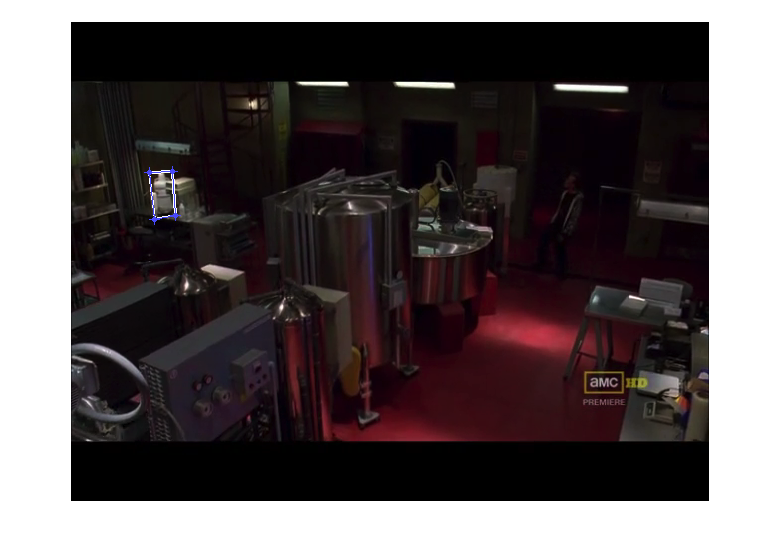
\includegraphics[width=\textwidth]{figures/region_queries/bb/selectionRegQ_52}
\end{subfigure}
\caption{Selected region (in blue) in a frame of the breaking bad data-set: a white tubus in frame 52.}
\label{fig:bb_regionquery_sel1}
\end{figure}

\begin{figure}[!htbp]
\centering
\begin{subfigure}{1.0\textwidth}
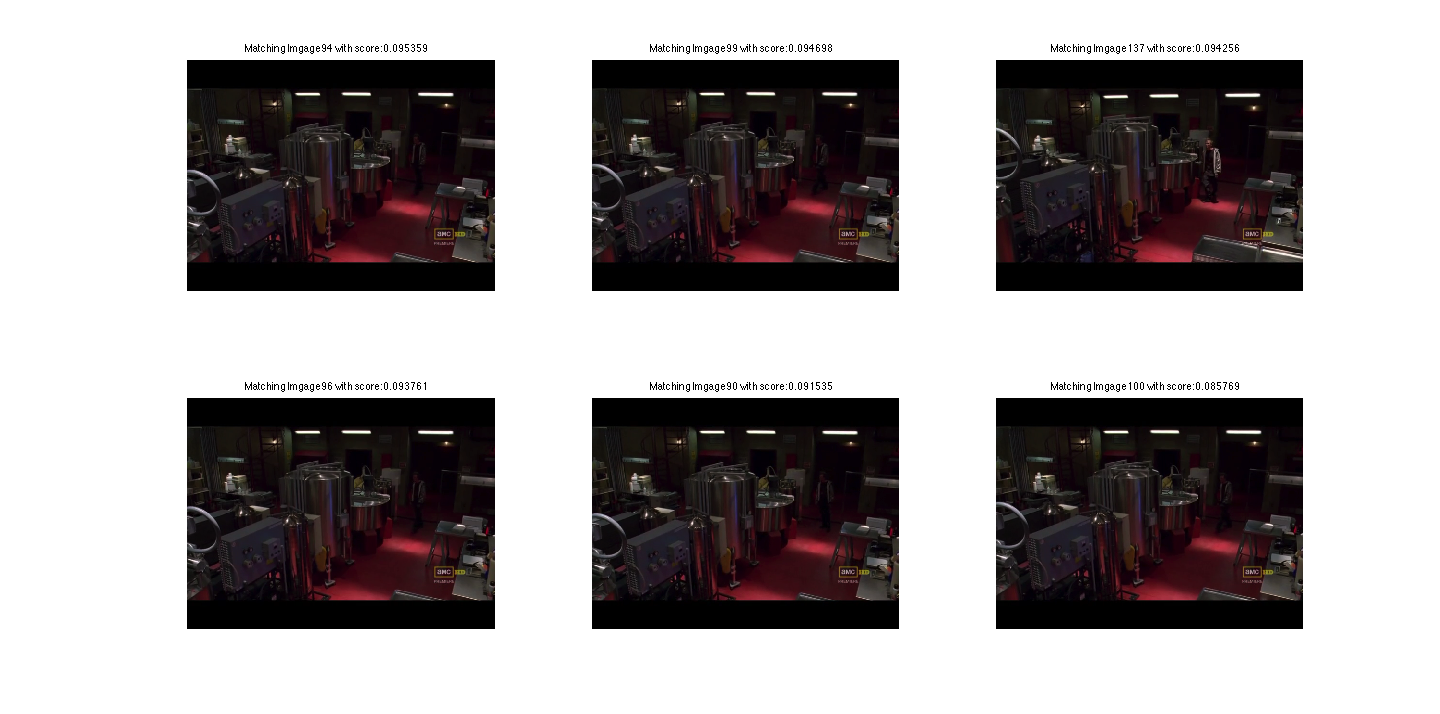
\includegraphics[width=\textwidth]{figures/region_queries/bb/matchesRegQ_52}
\end{subfigure}
\caption{Corresponding best matching frames when a user selects the white tubus in frame 52 of the breaking bad data-set.}
\label{fig:bb_regionquery_matches1}
\end{figure}

% breaking bad data set 2
\begin{figure}[!htbp]
\centering
\begin{subfigure}{1.0\textwidth}
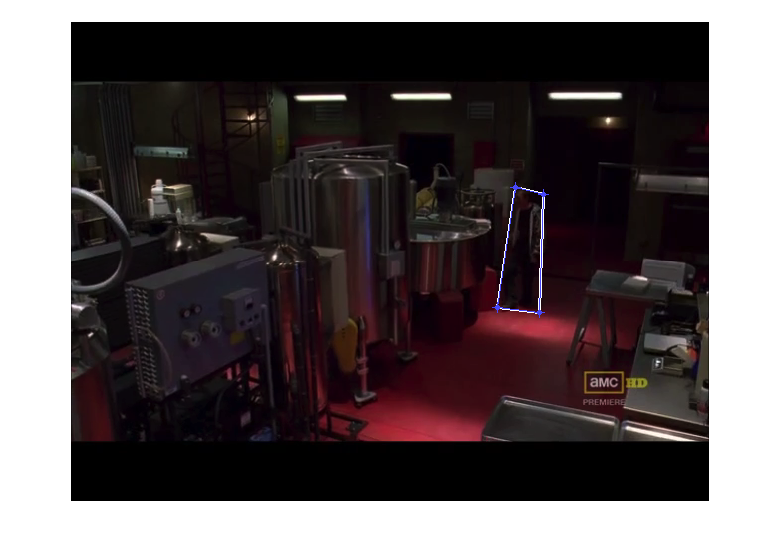
\includegraphics[width=\textwidth]{figures/region_queries/bb/selectionRegQ_125}
\end{subfigure}
\caption{Selected region (in blue) in a frame of the breaking bad data-set: Jesse (the man) in frame 125.}
\label{fig:bb_regionquery_sel2}
\end{figure}

\begin{figure}[!htbp]
\centering
\begin{subfigure}{1.0\textwidth}
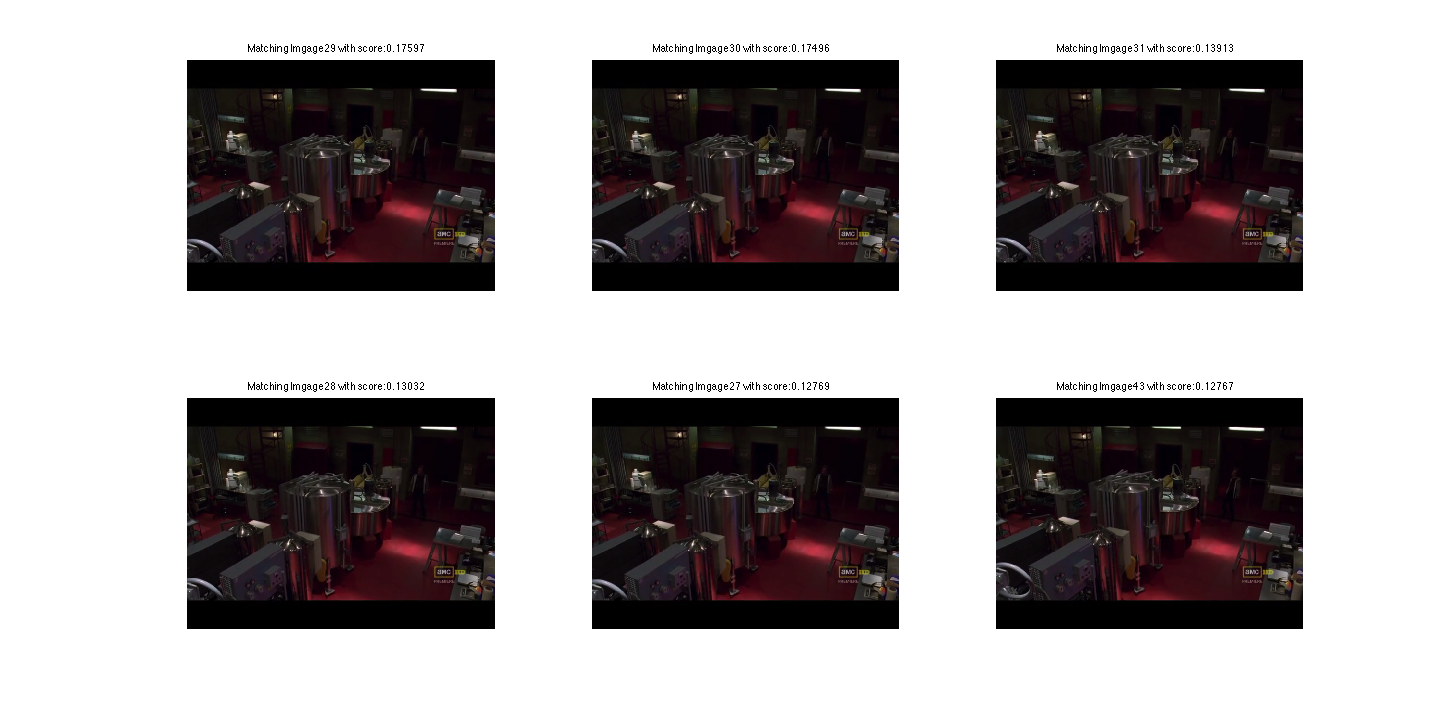
\includegraphics[width=\textwidth]{figures/region_queries/bb/matchesRegQ_125}
\end{subfigure}
\caption{Corresponding best matching frames when a user selects Jesse (the man) in frame 125 of the breaking bad data-set.}
\label{fig:bb_regionquery_matches2}
\end{figure}

% breaking bad data set 3
\begin{figure}[!htbp]
\centering
\begin{subfigure}{1.0\textwidth}
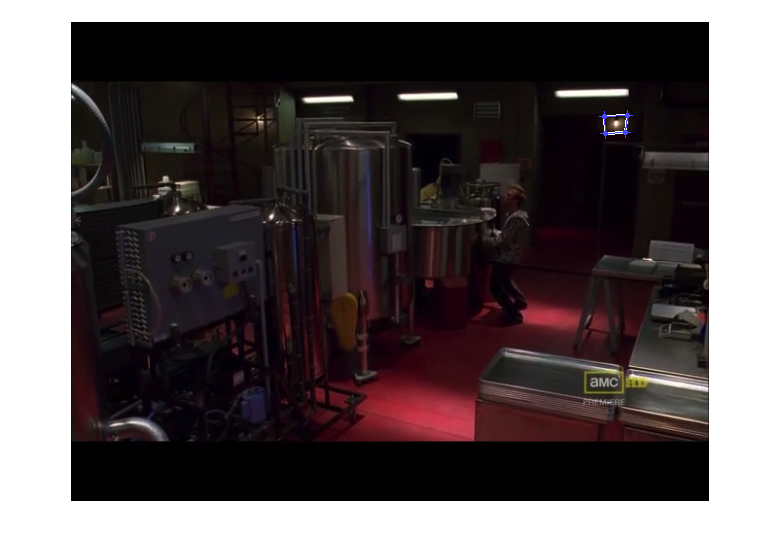
\includegraphics[width=\textwidth]{figures/region_queries/bb/selectionRegQ_180}
\end{subfigure}
\caption{Selected region (in blue) in a frame of the breaking bad data-set: the yellowish light in frame 180.}
\label{fig:bb_regionquery_sel3}
\end{figure}

\begin{figure}[!htbp]
\centering
\begin{subfigure}{1.0\textwidth}
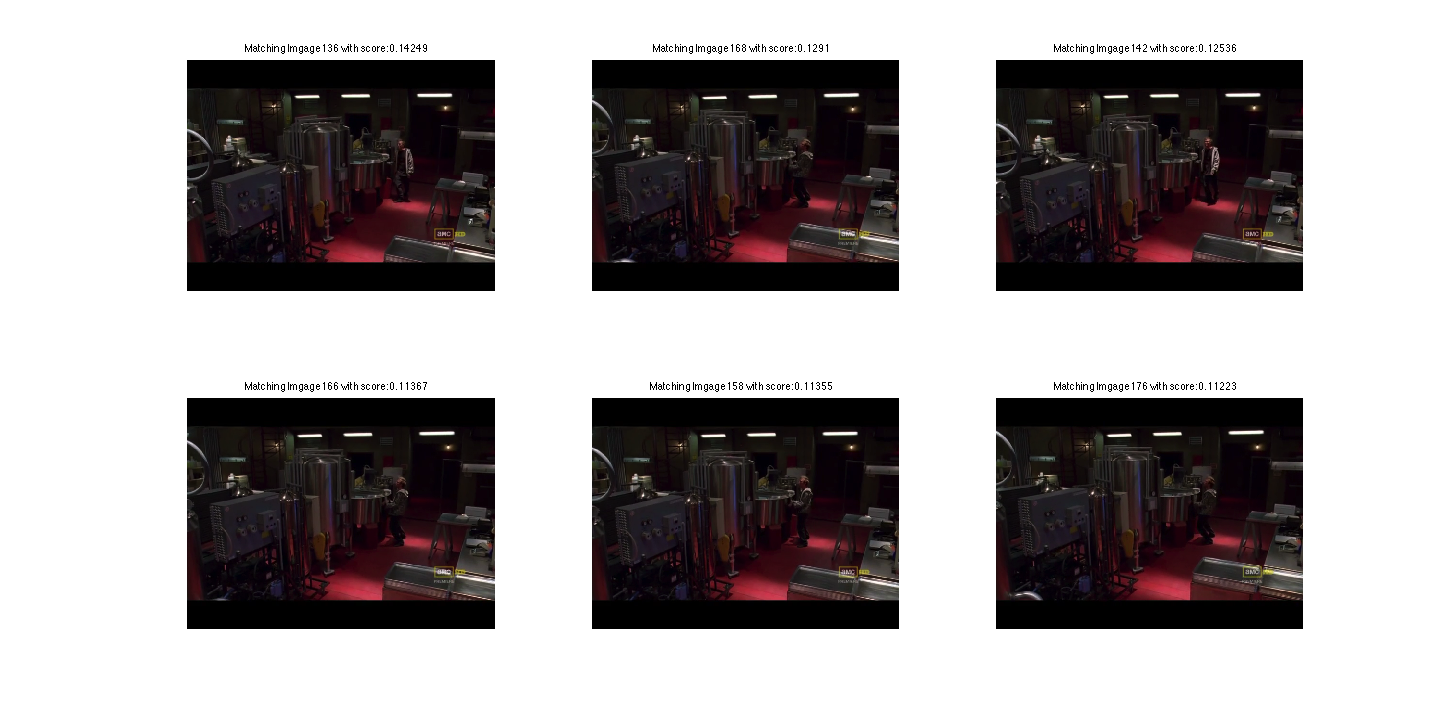
\includegraphics[width=\textwidth]{figures/region_queries/bb/matchesRegQ_180}
\end{subfigure}
\caption{Corresponding best matching frames when a user selects the yellowish light in frame 180 of the breaking bad data-set.}
\label{fig:bb_regionquery_matches3}
\end{figure}



% kids data set 1
\begin{figure}[!htbp]
\centering
\begin{subfigure}{1.0\textwidth}
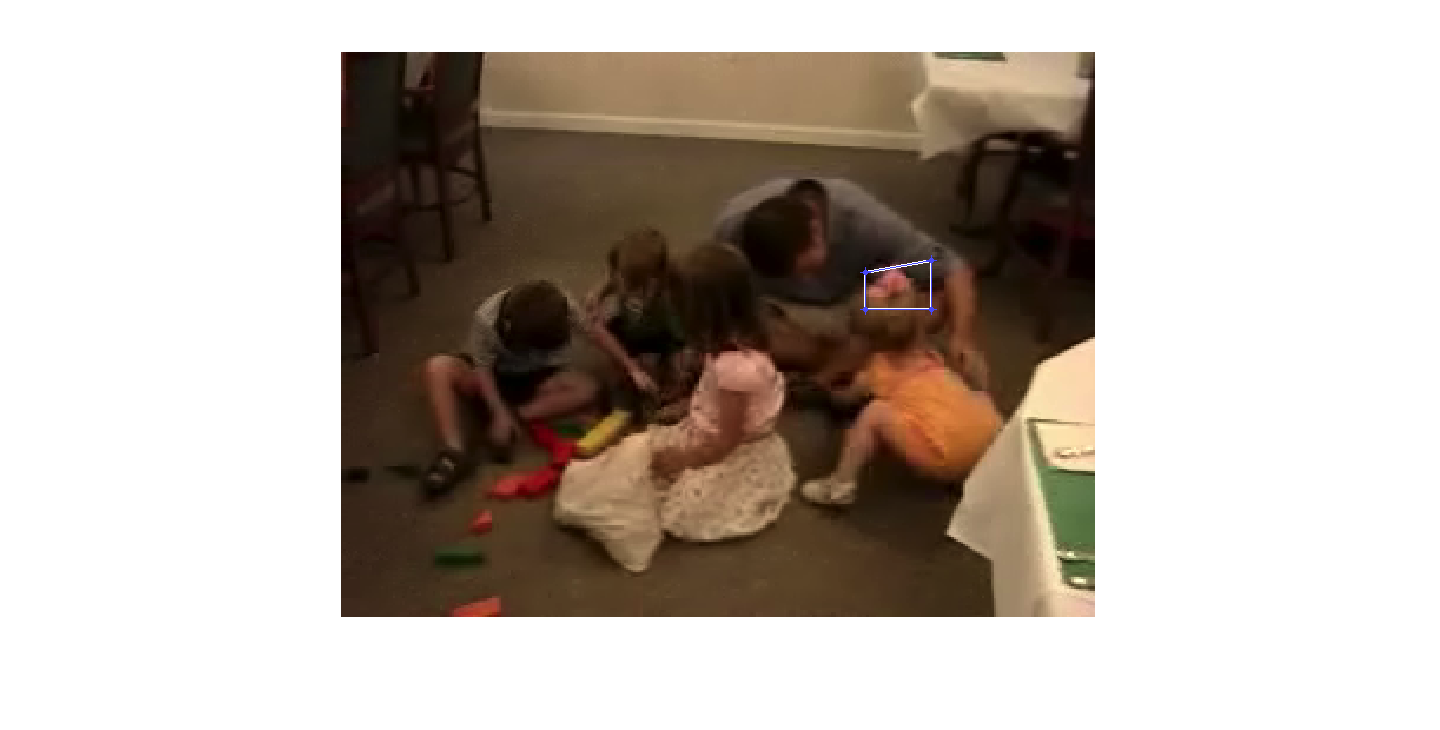
\includegraphics[width=\textwidth]{figures/region_queries/kids/selectionRegQ_94}
\end{subfigure}
\caption{Selected region (in blue) in a frame of the kids data-set: the girl's hairbow in frame 94.}
\label{fig:kids_regionquery_sel1}
\end{figure}

\begin{figure}[!htbp]
\centering
\begin{subfigure}{1.0\textwidth}
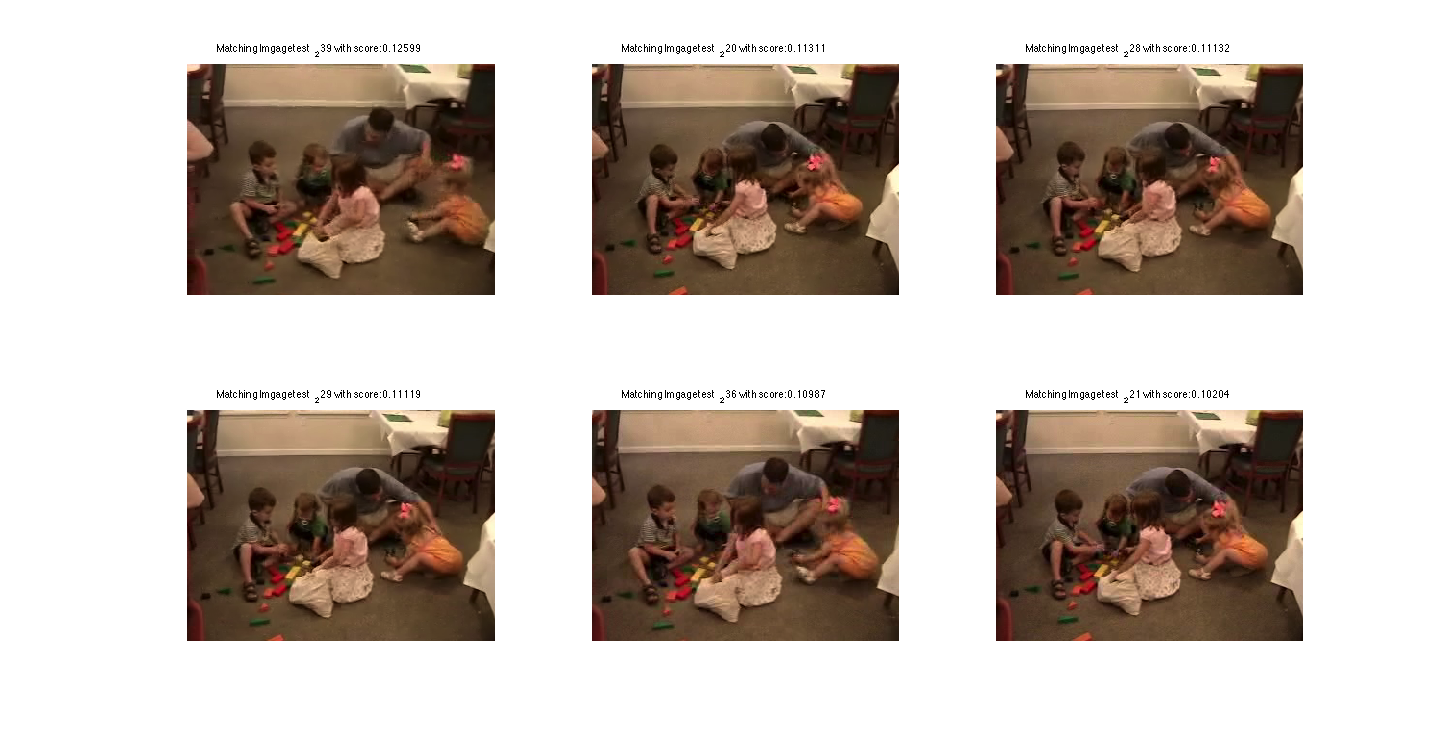
\includegraphics[width=\textwidth]{figures/region_queries/kids/matchesRegQ_94}
\end{subfigure}
\caption{Corresponding best matching frames when a user selects the girl's hairbow in frame 94 of the kids data-set.}
\label{fig:kids_regionquery_matches1}
\end{figure}


% kids data set 2
\begin{figure}[!htbp]
\centering
\begin{subfigure}{1.0\textwidth}
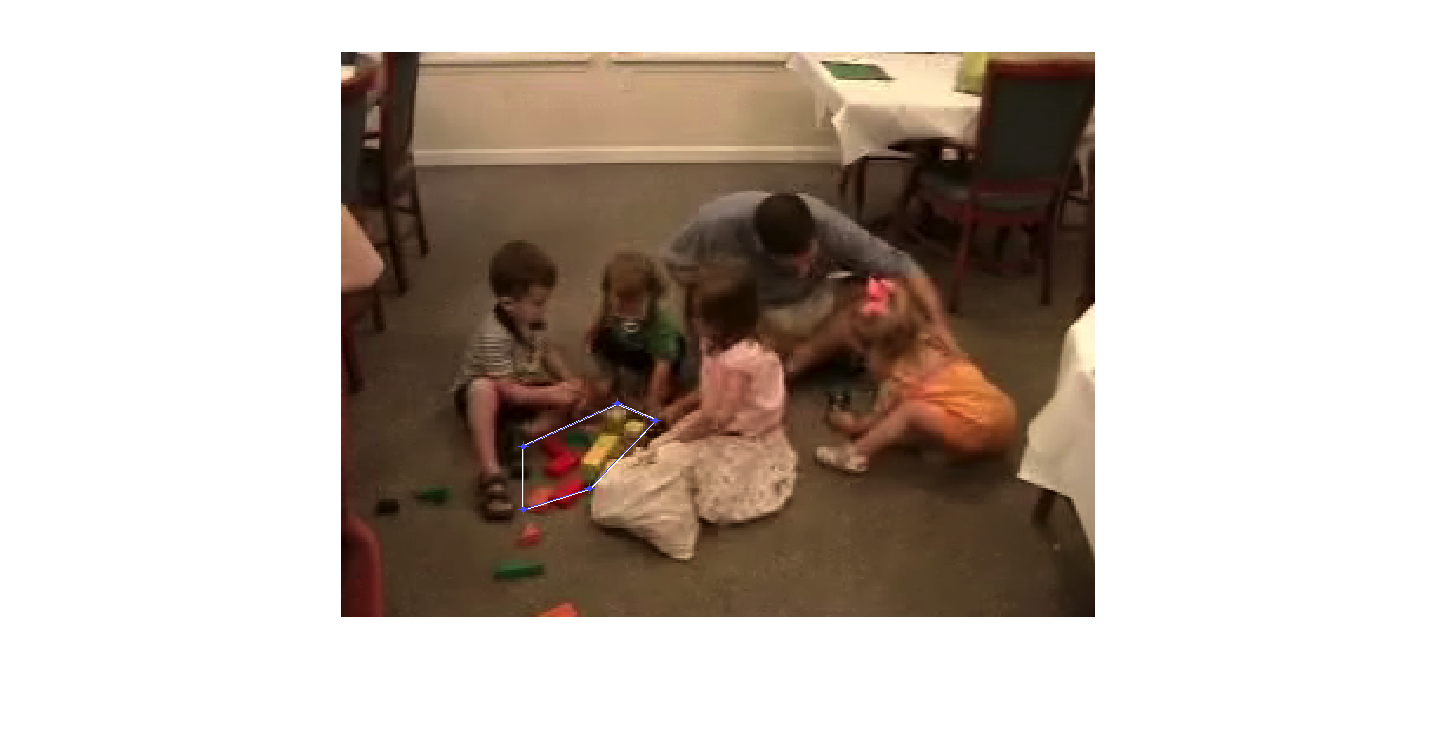
\includegraphics[width=\textwidth]{figures/region_queries/kids/selectionRegQ_230}
\end{subfigure}
\caption{Selected region (in blue) in a frame of the kids data-set: the kids' toys in frame 230.}
\label{fig:kids_regionquery_sel2}
\end{figure}

\begin{figure}[!htbp]
\centering
\begin{subfigure}{1.0\textwidth}
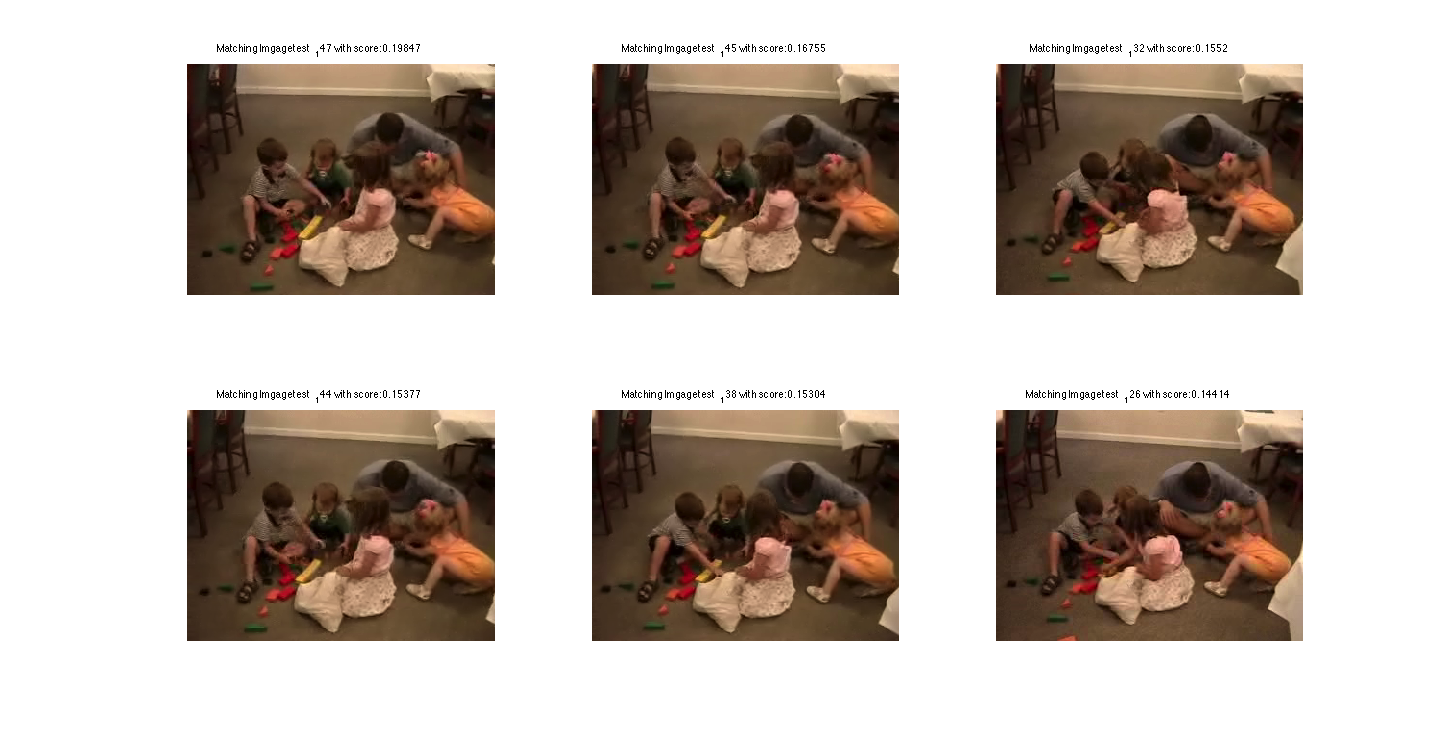
\includegraphics[width=\textwidth]{figures/region_queries/kids/matchesRegQ_230}
\end{subfigure}
\caption{Corresponding best matching frames when a user selects the kids' toys in frame 230 of the kids data-set.}
\label{fig:kids_regionquery_matches2}
\end{figure}


% kids data set Fail example
\begin{figure}[!htbp]
\centering
\begin{subfigure}{1.0\textwidth}
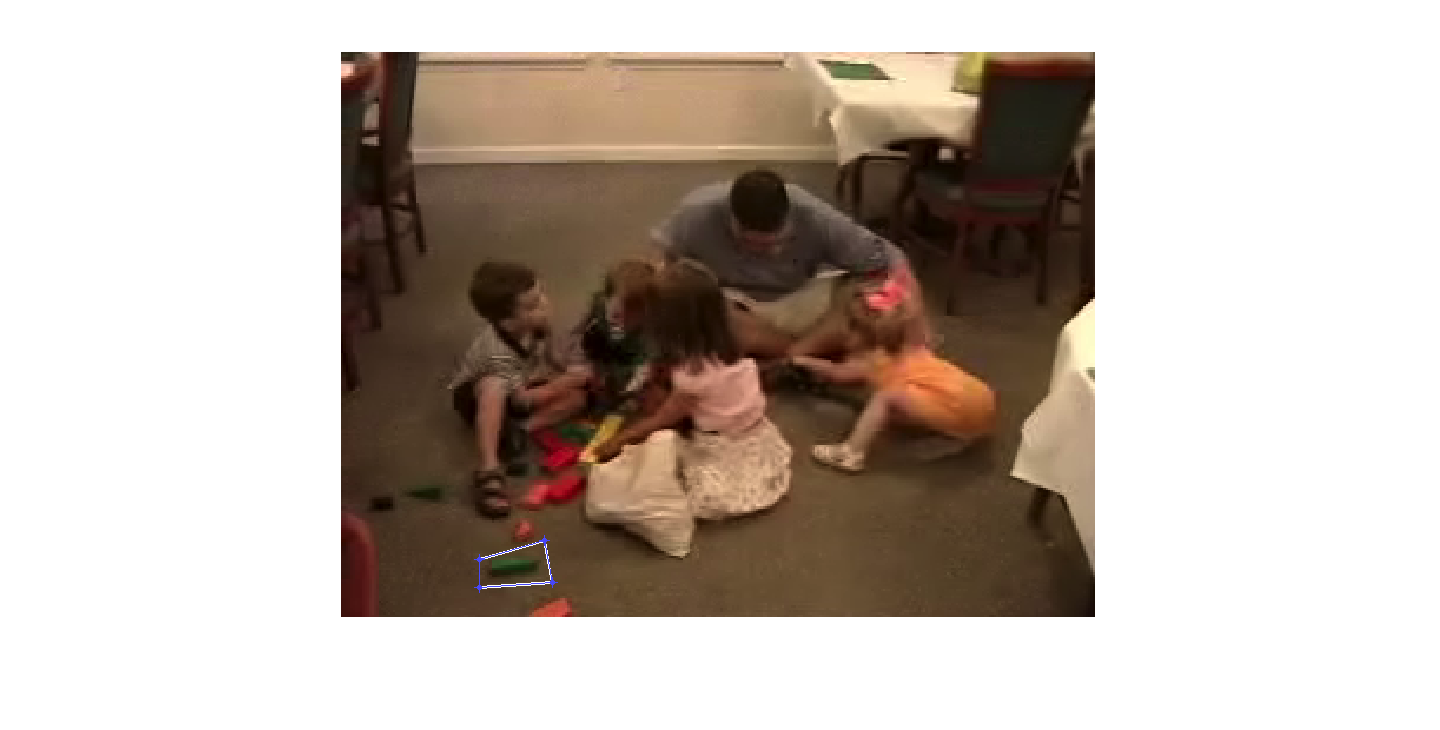
\includegraphics[width=\textwidth]{figures/region_queries/kids/selectionRegQ_204_fail}
\end{subfigure}
\caption{Selected region (in blue) in a frame of the kids data-set: the green small block toy in frame 204.}
\label{fig:kids_regionquery_sel3}
\end{figure}

\begin{figure}[!htbp]
\centering
\begin{subfigure}{1.0\textwidth}
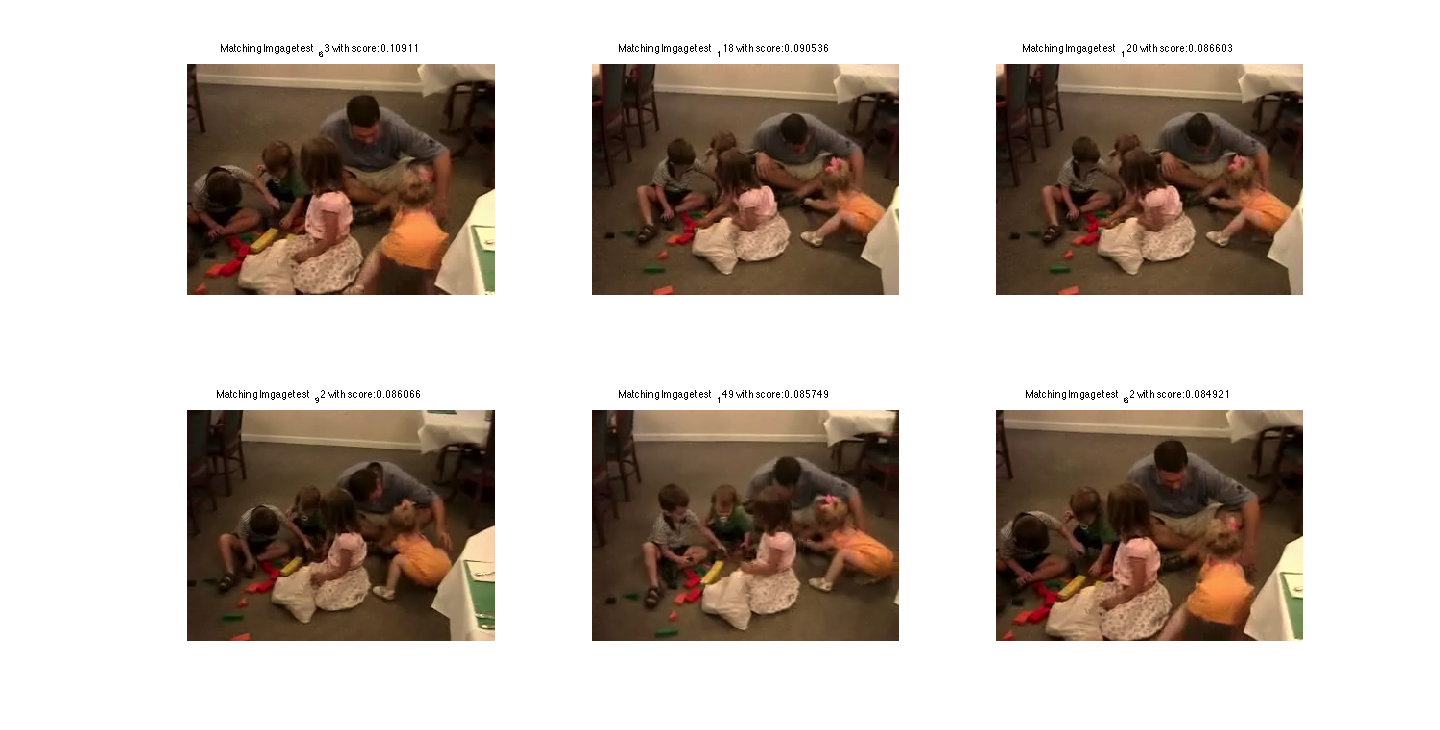
\includegraphics[width=\textwidth]{figures/region_queries/kids/matchesRegQ_204_fail}
\end{subfigure}
\caption{Corresponding best matching frames when a user selects he green small block toy in frame 204 of the kids data-set containing a missmatch. The last image includes no such shaped toy block.}
\label{fig:kids_regionquery_matches_fail}
\end{figure}

\end{document}